\section{ME21B190}
\subsection{Navier-stokes equation}
   
\begin{figure}[h]
\centering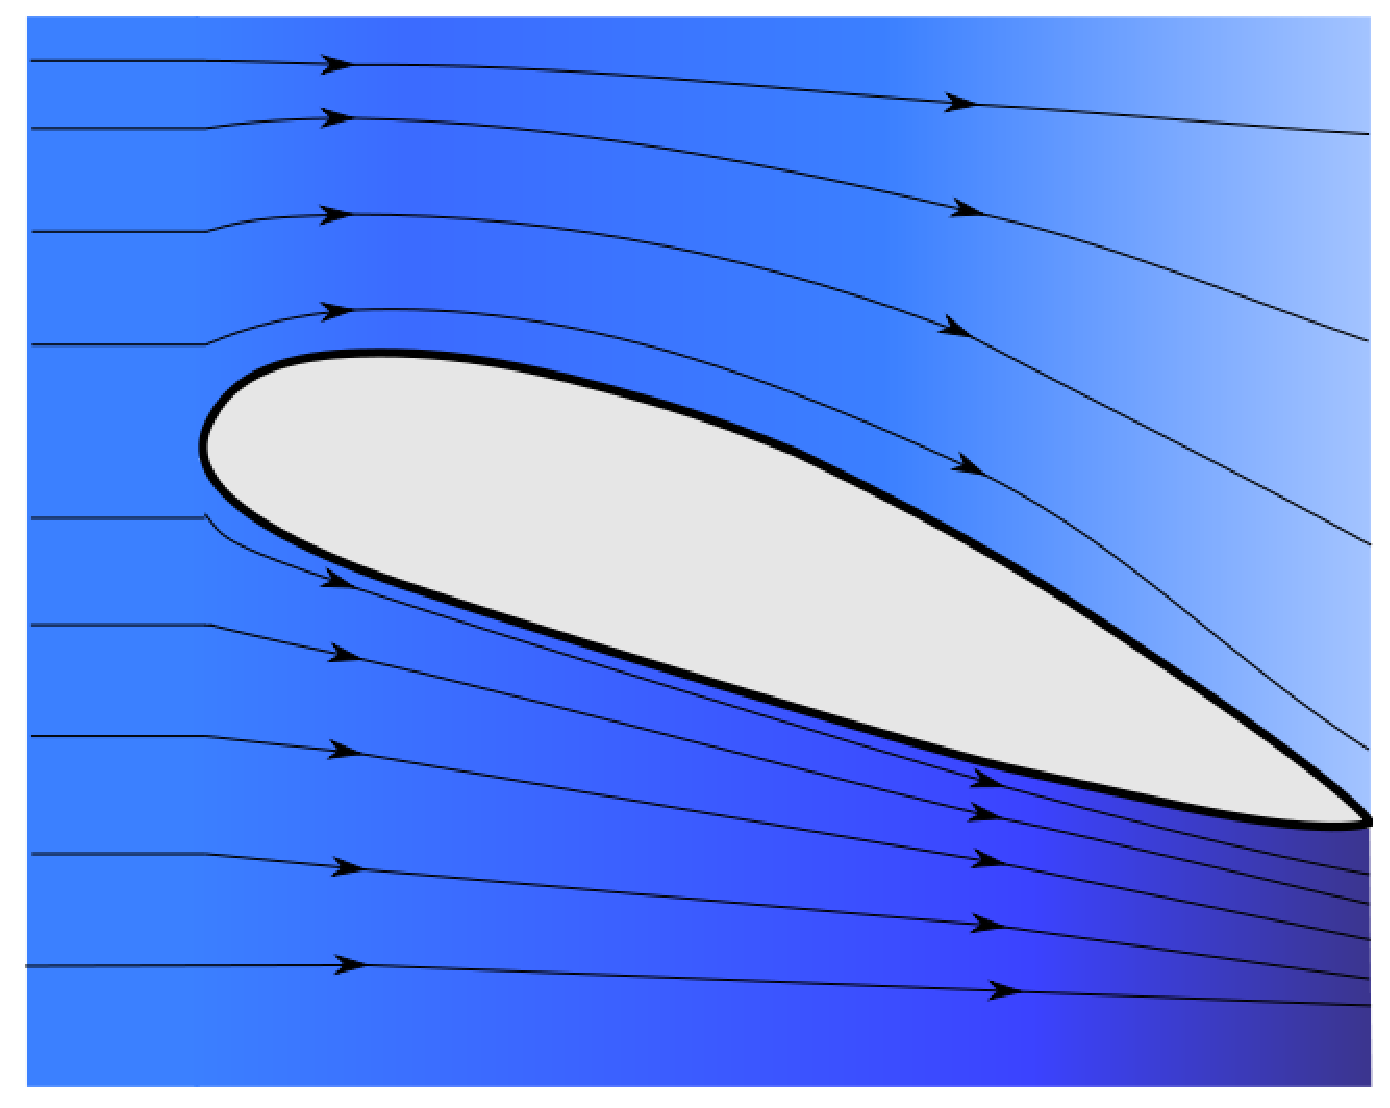
\includegraphics[width=0.5\textwidth]{./ME21B190/air.eps}
\end{figure}
\subsection{Continuity Equation:}

$$\nabla.\vec{V}=0$$


\large\ The countinuity equation describes the trasport of some quantities like fluid or gas.The equation explains how a fluid conserves mass in its motion.
\subsubsection {Momentum Equations:}

$$\frac{d\vec{V}}{dt}=\frac{\partial V}{\partial t} + (V.\nabla)V$$
\ Here the total derivative is the sum of change in velocity with time and the convective term
$$\rho\frac{d\vec{V}}{dt}=-\nabla{p} + \rho\vec{g}+\mu\nabla^{2}\vec{V}$$
 *The first term in RHS is the "Pressure gradient term" which tells in which direction the fluid flows

*The second term is the "Body force term",which includes all type of forces
*The third term "Diffusion term" 
\subsection{Explanation of variables}
\begin{center}
\begin{tabular}{ c c } 
   \hline
   \textbf{Symbol} & \textbf{Explanation} \\
   \hline
   $\vec{V}$ & velocity vector \\
   \hline
   $\rho$ & density of fluid \\
   \hline
   $\vec{g}$ & acceleration due to gravity \\
   \hline
   ${p}$ & pressure of fluid \\
   \hline
   $\mu$ & viscosity of fluid \\
   \hline
\end{tabular}
\end{center}
